% =====================================================================
%  SUPPLEMENTAL MATERIAL -- Radiology: Artificial Intelligence
%  Uploaded as a separate file. Anonymised on the same rules as main.tex:
%  no institution, no repository, no persistent identifier, no file path.
%
%  This holds the descriptive cross-study comparison, which was a
%  main-text figure in an earlier revision and is secondary here. It is
%  not inferential, no average is taken over it, and no claim in the
%  manuscript rests on it; it is retained because removing it entirely
%  would hide a comparison the earlier record contains.
%
%  Build: tectonic supplement.tex
% =====================================================================
\documentclass[11pt,letterpaper]{article}

\usepackage[T1]{fontenc}
\usepackage[utf8]{inputenc}
\usepackage{mathptmx}
\usepackage[margin=1in]{geometry}
\usepackage{graphicx}
\usepackage{siunitx}

\sisetup{group-separator={,},group-minimum-digits=4}
\pagestyle{empty}
\setlength{\parindent}{0pt}
\setlength{\parskip}{0.6em}

\begin{document}

\begin{center}
{\large\bfseries Supplemental Material\par}
{\small\itshape What a Slice-Level Benchmark Certifies without the Pixels:
An Audit of Six Public Imaging Datasets\par}
\end{center}

\vspace{0.6em}
\hrule
\vspace{1.0em}

\begin{center}
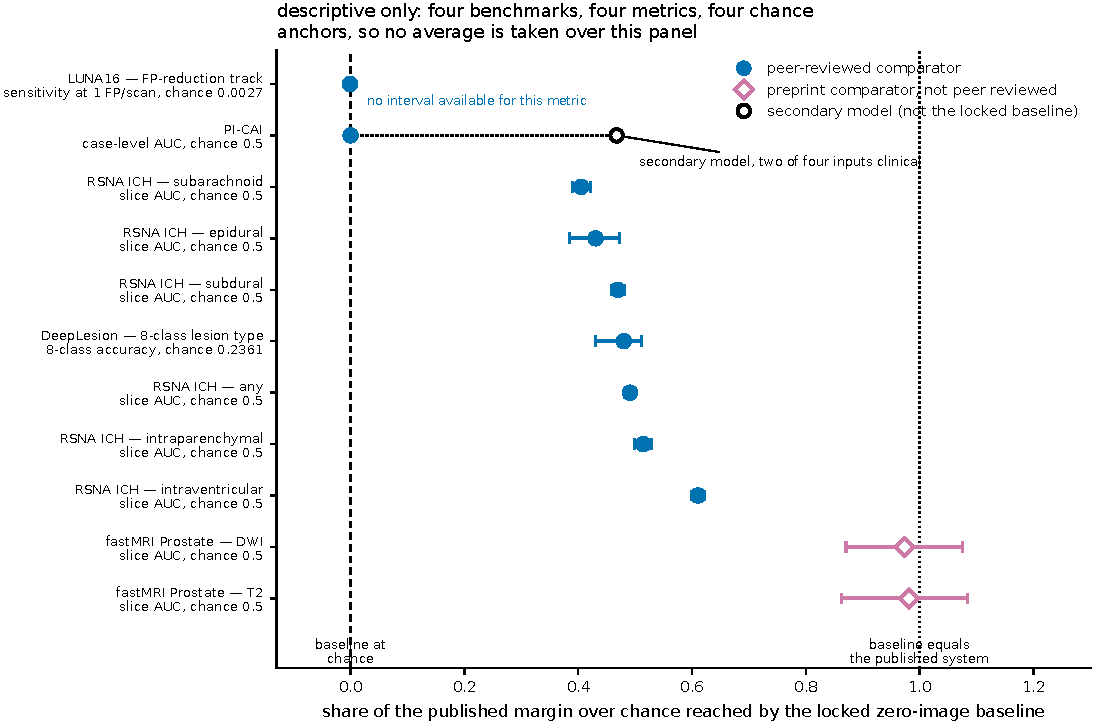
\includegraphics[width=\textwidth]{figures/figS1_trivial_fraction.pdf}
\end{center}

\textbf{Figure S1.} A descriptive cross-study comparison: the share of a published
margin over chance reached by the locked pixel-blind baseline, for the strongest
published comparator on each benchmark. This is not an inferential quantity and
no average is taken over the panel. The four peer-reviewed benchmarks sit on four
different metrics against four different chance anchors, printed on each row, and
they run from about half the published margin to none of it; that spread is the
finding. Error bars are 95\% subject-clustered bootstrap intervals propagating
uncertainty in the baseline only. Rows whose comparator is a preprint that has
not been peer reviewed are marked as such and are the two highest here, at 0.981
and 0.973. LUNA16 is plotted at $-0.001$, computed on the frozen holdout from
sensitivity at one false positive per scan and not from the challenge's
competition performance metric; the reference used in place of 0.5 is the
random-score value of that metric on the same held-out scans. No interval is
available for that row. PI-CAI is plotted at 0.174, read at the case unit from
the locked positional baseline fitted on its lesion delineation volumes and mean
aggregated. An earlier revision reported this row as not estimable, which was
true of that benchmark's public marksheet---it carries no slice index---and false
of the benchmark, whose delineation volumes supply one. That row is across
cohorts: the published comparator is on the hidden test set and the baseline is
on the development set. The open marker on the same row is its secondary tree
over four non-image columns, two of which are clinical predictors rather than
acquisition fields, and is not part of this comparison.

\end{document}
